% Chapter 4

\chapter{Results} % Main chapter title

\label{Chapter4}  

\section{Artefact}
The artefact that was developed is a computer game and is titled \textit{"Puzzle Ball: Spherical Shadows"} and is a self-contained application that can be launched standalone without any additional software needed. While it is fairly lightweight on hardware resources for a computer game, it does require more resources than a typical application and may stutter on older systems due to the effects used. In terms of the genres it encompass, it would full under the platformer, puzzle and action genres for games and as such is described as a 3D puzzle platformer with aspects of action gameplay played in first person.
\\\\
Once the application is launched, the user is taken to the \textit{Main Menu} screen (depicted below) where clicking the text \textit{Play} triggers a function to start the first level - that being the the Tutorial. Each group member was responsible for the design of an individual level where the Tutorial/First level being the level undertaken in this project. The reason for this is that the research aspect of this project aligns with the goals of a tutorial level. 

\begin{figure}[H]
\centering
\begin{subfigure}{0.5\textwidth}
  \centering
  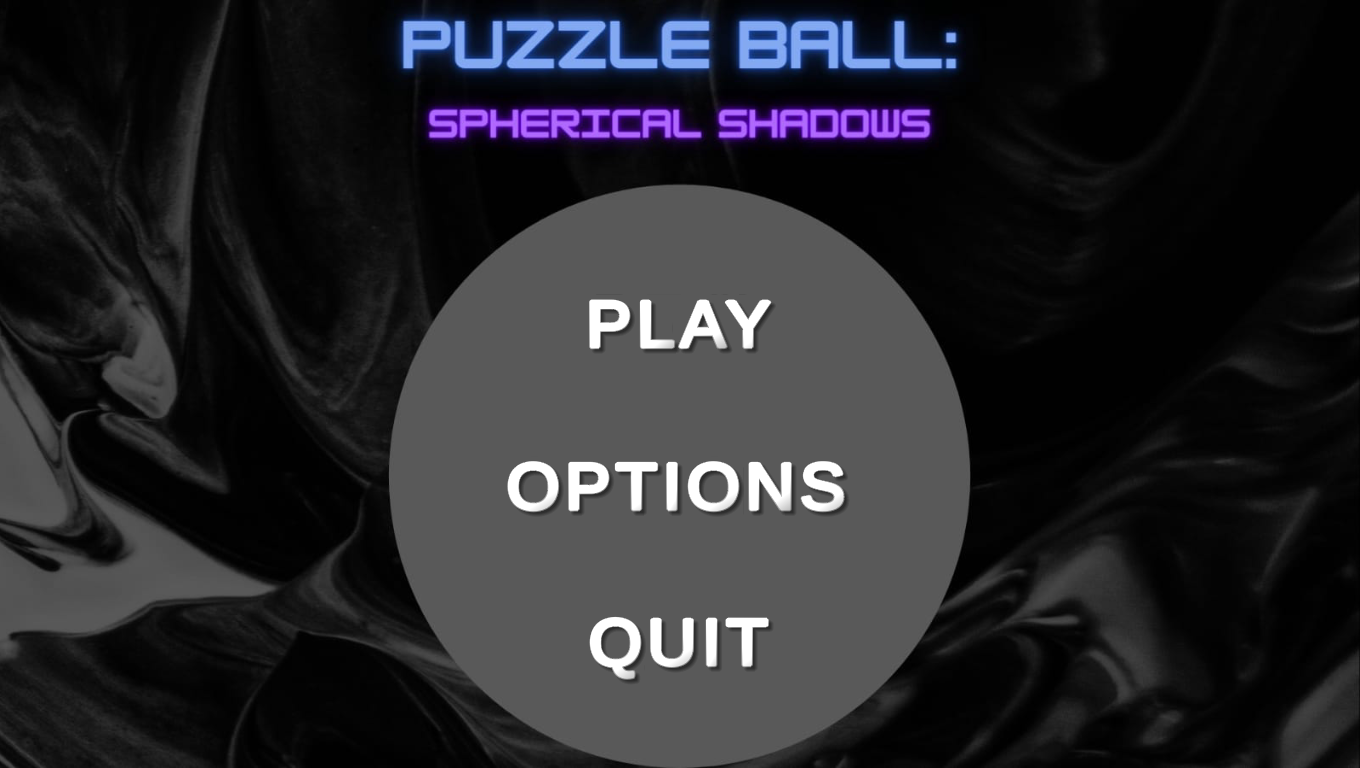
\includegraphics[width=1\linewidth]{Figures/menu.png}
  \caption{The Main Menu of the Artefact}
\end{subfigure}%
\begin{subfigure}{0.5\textwidth}
  \centering
  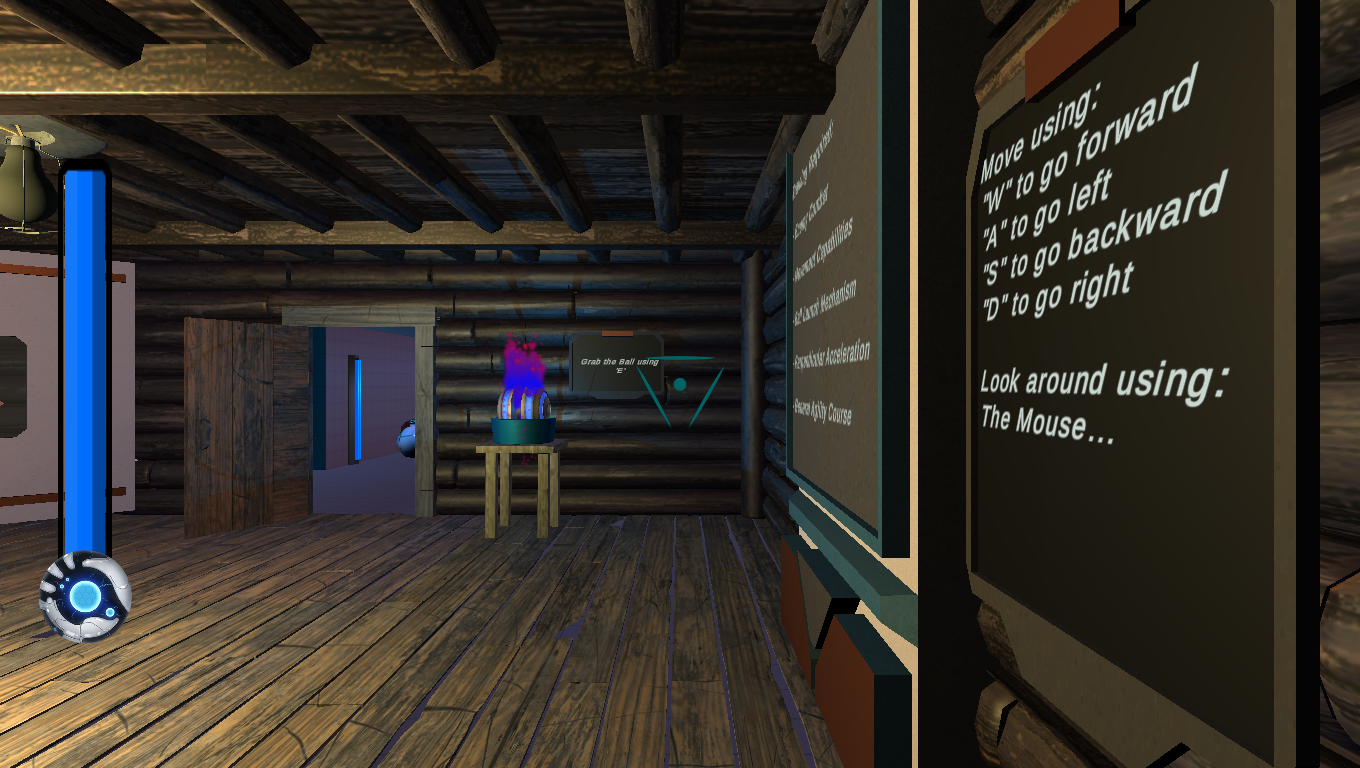
\includegraphics[width=1\linewidth]{Figures/start.png}
  \caption{The Starting Point of the Level}
\end{subfigure}
\caption{Starting the Game}
\end{figure}

\noindent One the tutorial level has started, the user is shown the basic character movement controls on the right side of the screen and can continue forward. Text based signs were used throughout the level to explain various mechanics or tasks to be completed - an example of this is shown in Figure 4.2 below.

\begin{figure}[H]
\centering
\centerline{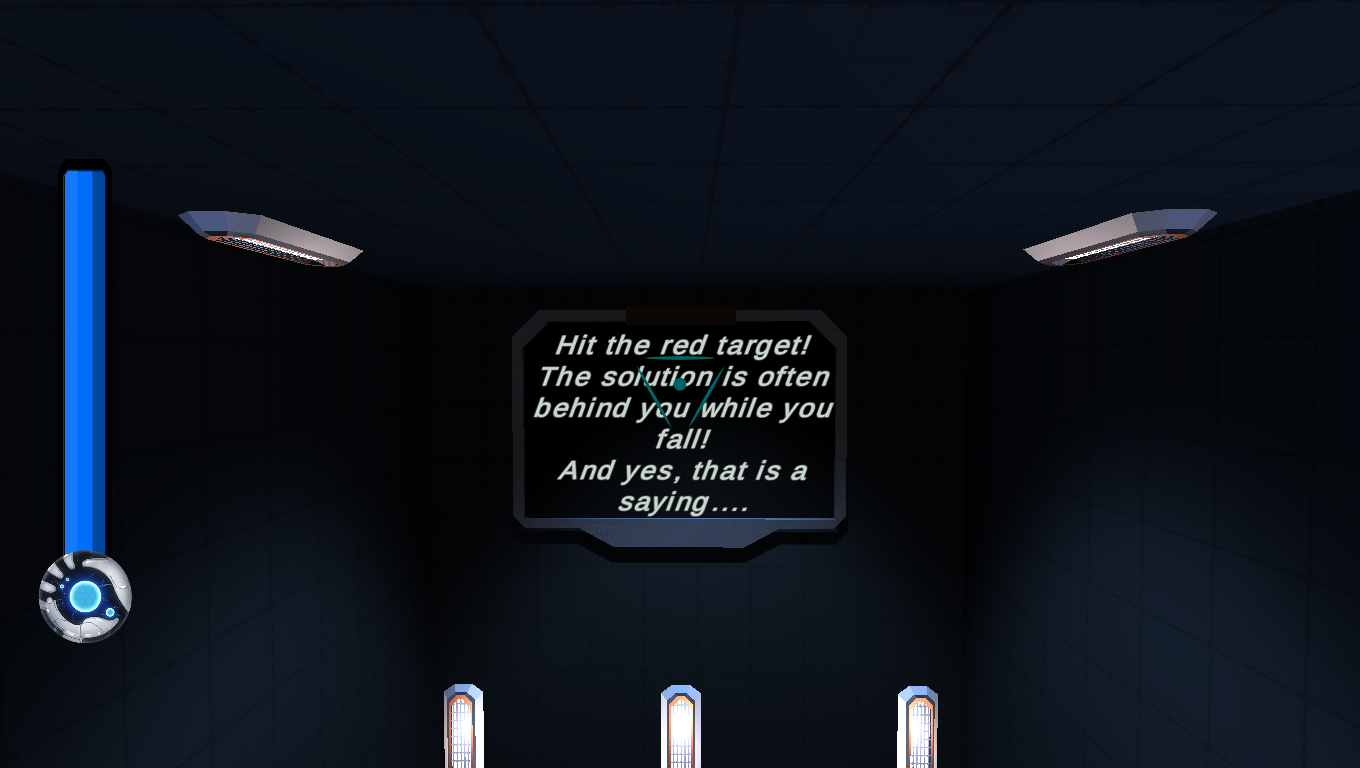
\includegraphics[scale=0.33]{tutSignEg.png}}
\caption{A Further Example of the Tutorial Signs}
\end{figure}

\noindent The user must then make there way to a central area, referred to as the Hub Room, where they are given the choice in what order they would like to complete the five main tutorials. These will be discussed and shown below. As the user completes the several tutorials, a blockade that restricted movement to the next level is slowly removed as shown below.

\begin{figure}[H]
\centering
\begin{subfigure}{0.3\textwidth}
  \centering
  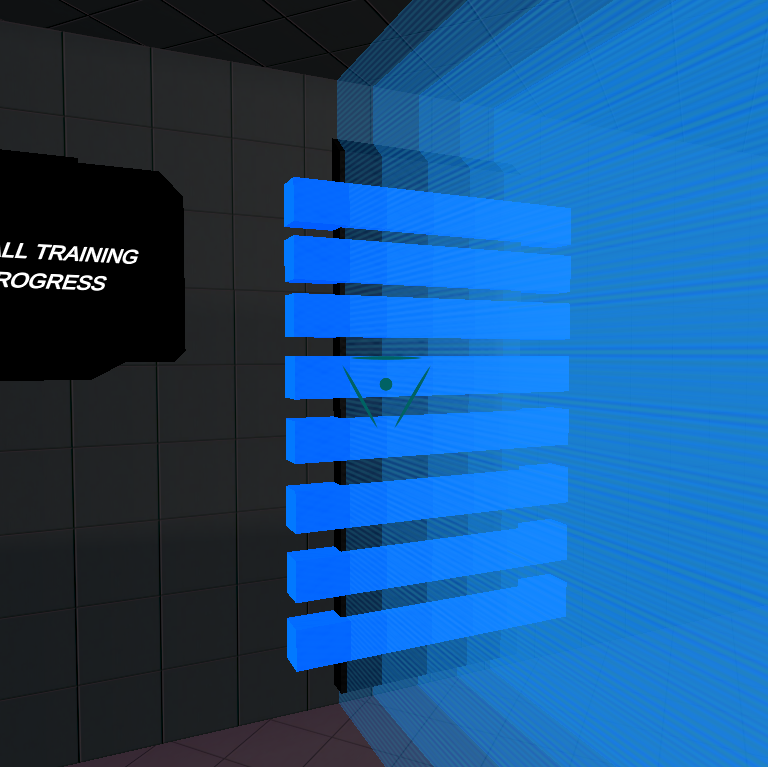
\includegraphics[width=0.9\linewidth]{Figures/barrier5.png}
  \caption{No Tutorials Completed}
\end{subfigure}%
\begin{subfigure}{0.3\textwidth}
  \centering
  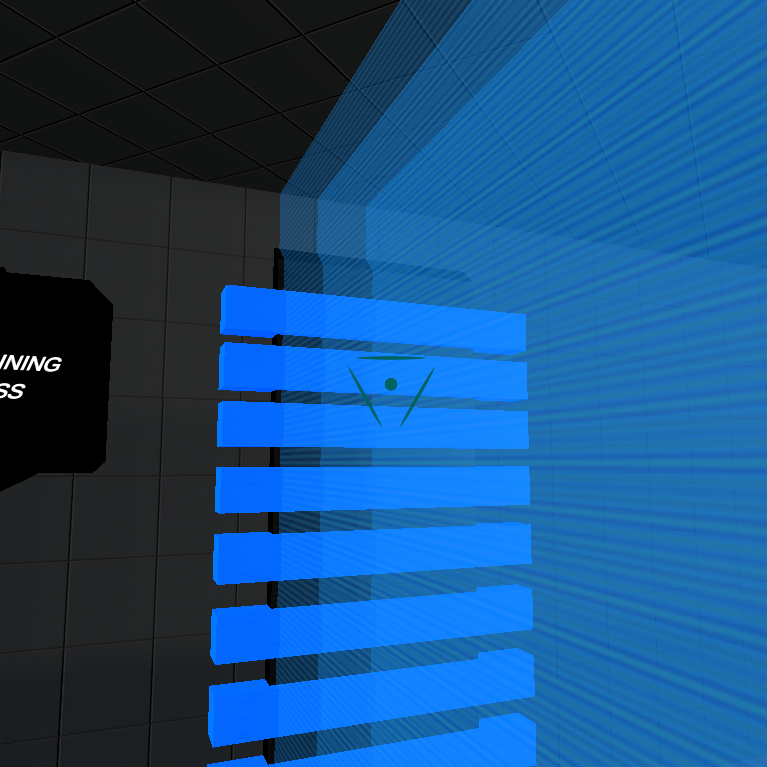
\includegraphics[width=0.9\linewidth]{Figures/barrier3.png}
  \caption{Two Tutorials Completed}
\end{subfigure}
\begin{subfigure}{0.3\textwidth}
  \centering
  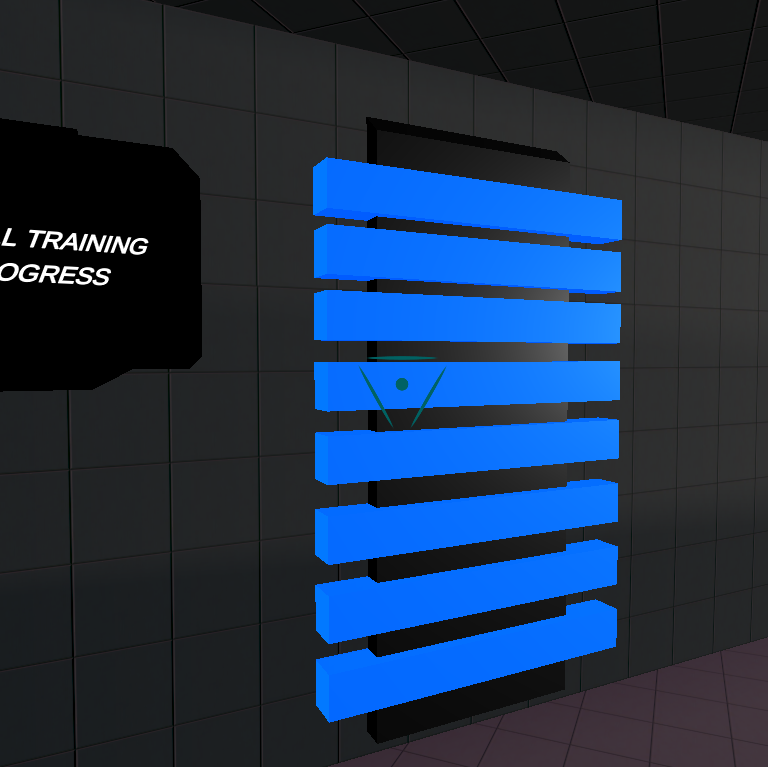
\includegraphics[width=0.9\linewidth]{Figures/barrier0.png}
  \caption{All Tutorials Completed}
\end{subfigure}
\caption{Progress Blocker in Tutorial}
\end{figure}

\noindent Once all the tutorials in this level are completed and the blockade removed, the user is allowed to move towards the final room where they must throw the ball object into the centre of the desk-like object with a particle effect on it.

\begin{figure}[H]
\centering
\centerline{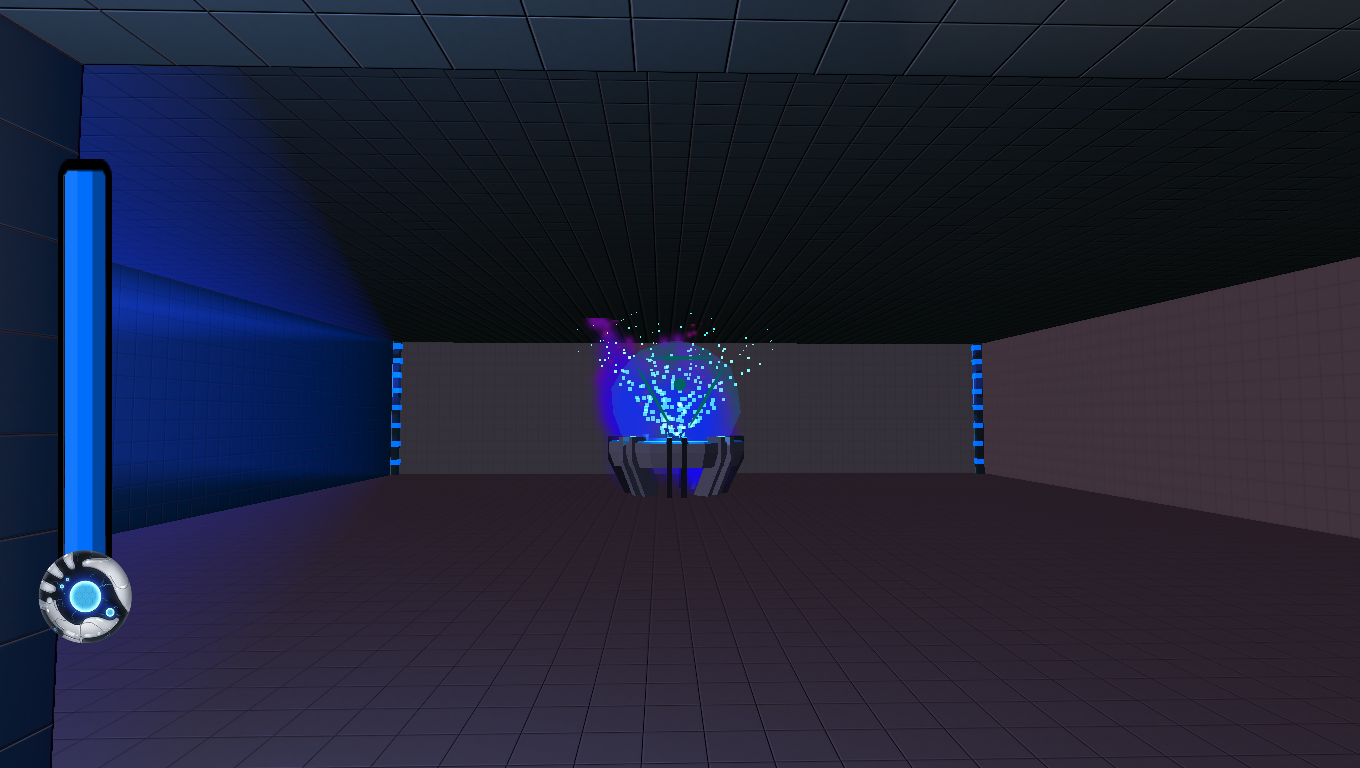
\includegraphics[scale=0.33]{Figures/endgoal.png}}
\caption{The End Goal Object}
\end{figure}

\noindent Once the ball object collides with the end goal object, the user is taken to the next level where the main aim to to traverse the level and throw the ball object into the next end goal. This process is followed for two additional levels for three in total  after which the user is taken to a scene where the group members and their contributions are listed with a prompt to close the application.

\begin{figure}[H]
\centering
\centerline{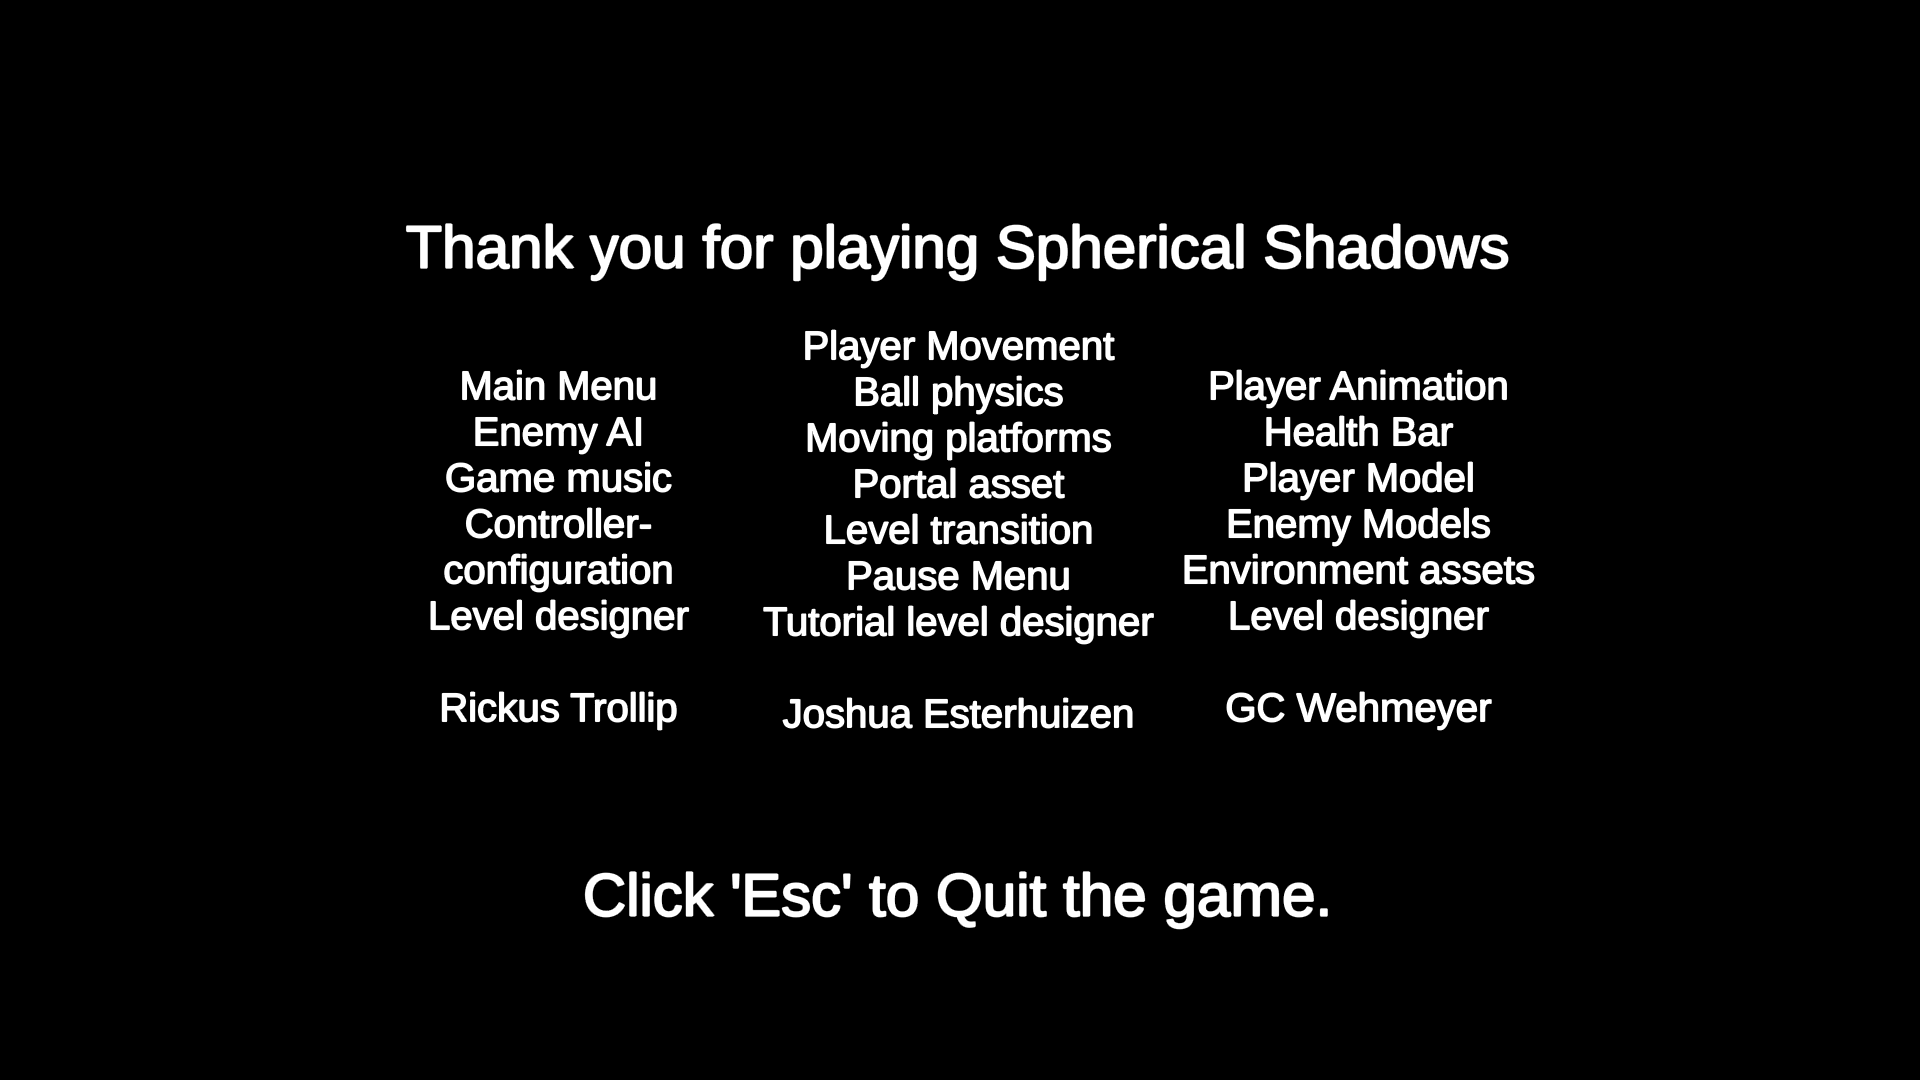
\includegraphics[scale=0.25]{Figures/credits.png}}
\caption{The Credits Screen}
\end{figure}

\noindent A list of all assets made use of during the development of the artefact, such as models and music, can be found on the GitHub repositories\footnote{\url{https://github.com/GCWehmeyer/Spherical_Shadows/blob/main/References.txt}}$^{,}$\footnote{\url{https://github.com/Josh-SCG/Spherical_Shadows/blob/main/References.txt}} 
\section{Article}
The individual research aspect of this project yielded a academic article titled \textit{"Linking Gamification, Ludology and Pedagogy: How to Use Serious Games for Various Knowledge Domains"}.
\\\\
A literary analysis on the fields of pedagogy, ludology and gamification was conducted and an article written in order to answer the question posed; \textit{What qualities and principles can be applied to a video game to allow it to be used in a learning environment as a means to provide better engagement among certain students by providing an enjoyable delivery of information?} This question was then refined and phrased as \textit{What qualities are required for a serious game to be effectively used in an educational environment on various topics?} within the article.
\\\\
The results of the research aspect of this project is the answer to these questions which were synthesised from various case studies and the literature analysis conducted. The literature study of the article is similar to the one conducted in this document with the addition to an analysis of three case studies in detail, one of which was mentioned in the literature study above in Chapter \ref{Chapter2}.
\\\\
The three case studies made use of are all titled:
\begin{itemize}
\item \textit{"Choose your own training adventure: designing a gamified SETA artefact for improving information security and privacy through interactive storytelling"}
\item \textit{"Anti-phishing phil: the design and evaluation of a game that teaches people not to fall for phish"}
\item \textit{"Children’s Awareness of Digital Wellness: A Serious Games Approach"}
\end{itemize}

\noindent Each case study was analysed to determine how the serious games were developed and which principles, qualities or frameworks were a large contributing factor to the development. A summary of the findings from the case studies alone is shown in Table \ref{tab4.1}

\begin{table}[H]
\caption{Design Principles Defined by Case Study (\cite{Dincelli2020,Sheng2007,allers2021children})}
\begin{center}
\begin{tabular}{|c|c|c|c|}
\hline

\textbf{SETA Artefact} & \textbf{\textit{Anti-Phishing Phil}}& \textbf{\textit{Happy Hippo}} \\
\hline
Story-based	& Story-based 			& Simplicity  \\
Reflection	& Reflection			& Clear and Simple Goals  \\
Feedback	& Feedback 				& Quality of Feedback and Rewards  \\
	-		& Conceptual-Procedural	& Structure of the Challenge  \\
	-		& 		-				& Motion-based Interaction  \\
\hline

\end{tabular}
\label{tab4.1}
\end{center}
\end{table}

\noindent In addition to these, qualities were derived from several educational theories discussed in the literature study as well as the findings section of the article. These include Merrill's First Principles, the ARCS model for motivation and a framework specific to teaching preschool children.
\\\\
The results of this encompass four archetypal qualities needed as well as a few qualities recommendations needed to be taken into account depending on the knowledge domain a topic falls under. The reasoning for choosing these specific qualities and recommendations is elaborated in detail in the article itself which can be found in Appendix \ref{AppendixC}. In short these qualities are named:
\begin{enumerate}
\item Reflection
\item Feedback
\item Story-telling
\item Structuring
\end{enumerate}


\noindent Reflection is described and giving a user enough time after they have completed a task or presented with new knowledge to think about it on their own without further instruction.
\\\\
The next quality is Feedback. Users should be given feedback on how they are progressing on a given set of tasks within the game at some point. Feedback should also be scaled up or down depending on how a user is progressing - that is, if a user is doing well they require less feedback on where to improve as compared to another user who may be struggling and should require more feedback on how to improve. Further than this, the means of presenting feedback is heavily dependant on the topic being taught, how tasks are handles and the general loop of the game. In addition to this. Feedback also includes the stipulation that the game should foster an environment of smaller accomplishments to keep users engaged with the game.
\\\\
Story-telling is also an important quality which centres around keeping engagement with the game high. It entails making use a story or role-play within the game or the use of a story-based agent such as a character that would guide users through the material and tasks. This can be done through contextual story-telling by having the tasks form part of a story's progression or as the main means of relaying information on a topic.
\\\\
The next quality encompasses a major part of the design of the game. Structuring refers to both the overall design of a serious game as well as how the tasks within it are designed. This quality has several key requirements that should be met for the most optimal experience by a user. Goals and expectations should be made simple and clear to a user from the beginning. Tasks and problems within the game should also scale in difficulty depending on a user's skill and progression - that is, when a user is struggling the tasks should be made easier until they demonstrate understanding with them upon which the difficulty is increased. A serious game in this context should also be designed around the topic making the information or tasks and problems the main focus of the game.
\\\\
While the above qualities are intended for use in any serious game being developed, the following section details certain recommendations for various knowledge domains. The definitions for each of these was also given in the literature study in Chapter \ref{Chapter2}.
\\\\
Both Hi-fidelity and low fidelity simulation games, these being a subset of serious games, are the most useful for teaching content found in the Affective, Soft Skills and Psychomotor domains since the best means to teach these is through immersing the user in the phenomena, repeated application of skills and observation respectively. Simulation-type serious games can also be used in the other domains such as with the game used to aid in teaching physics. These types of games are also the most effective means for the Psychomotor domain.
\newpage
\noindent The remaining knowledge domains tend to have some heavy overlap depending on the topic being covered. The Conceptual-Procedural principle is an example of this. To reiterate, it simply states that a topic cannot be fully understood from only the procedures or context - both are needed for a deeper understanding. As such if a topic where to fall under these domains it is vital to present information in a manner that all aspects are clear to a user.

\section{Conclusion}
This section dealt with the results generated as part of this research project. This included a digital computer game as well as various qualities needed in order for a serious game to be effectively used in an educational environment. In brief, these qualities were, Reflection, Feedback, Structuring and Story-telling. 